\documentclass[a4paper, 10pt]{article}
\usepackage[utf8]{inputenc} % Change according your file encoding
\usepackage{graphicx}
\usepackage{url}
\usepackage{amsmath}
\usepackage{amsfonts}
\usepackage{bbm}
\usepackage{amsthm}
\usepackage{tikz}
\usepackage[a4paper, left=2cm, right=2cm, top=2cm, bottom=2cm]{geometry}

\newtheorem{obs}{Observation}
\newtheorem{theorem}{Theorem}

\theoremstyle{definition} % amsthm only
\newtheorem{definition}{Definition}

%\newtheorem{def}{Definition}

\begin{document}

Team Bearland: Mart\'in, V. and Oviedo, P. and Segarra, C \hfill Tuesday, November 19th

\vspace{15pt}

\textbf{\Large Discrete and Algorithmic Geometry: Sheet 1}

\vspace{20pt}

\textbf{\textit{(1) True or false?}}

\vspace{3pt}

\hspace{5pt} \textbf{\textit{(a) This notion of contraction agrees with the notion of contraction in graph theory.}}

\vspace{3pt}

\hspace{5pt} \textbf{\textit{(b) $M_{G^\star} = \left(M_G\right)^\star$, if G is a planar graph and $G^\star$ its dual planar graph.}}

\vspace{10pt}

\textbf{\textit{(2) Prove that if a matroid M is realizable over a ground field $\mathbbm{k}$, then the dual matroid $M^\star$ is also realizble over $\mathbbm{k}$.}}

\vspace{10pt}

\textbf{\textit{(3) Consider the matroid M realized by the columns of the matrix}}
$$
\left[
    \begin{array}{ccccc}
        0 & 1 & 1 & 0 & 1 \\
        1 & 0 & 1 & 0 & 1 \\
        0 & 1 & 1 & 1 & 0
    \end{array}
\right]
$$
\textbf{\textit{ Compute a realization of $M^\star$, and some contractions of M of your choosing.}}

\begin{figure}[h!]
    \centering
    \resizebox{.8\linewidth}{!}{
        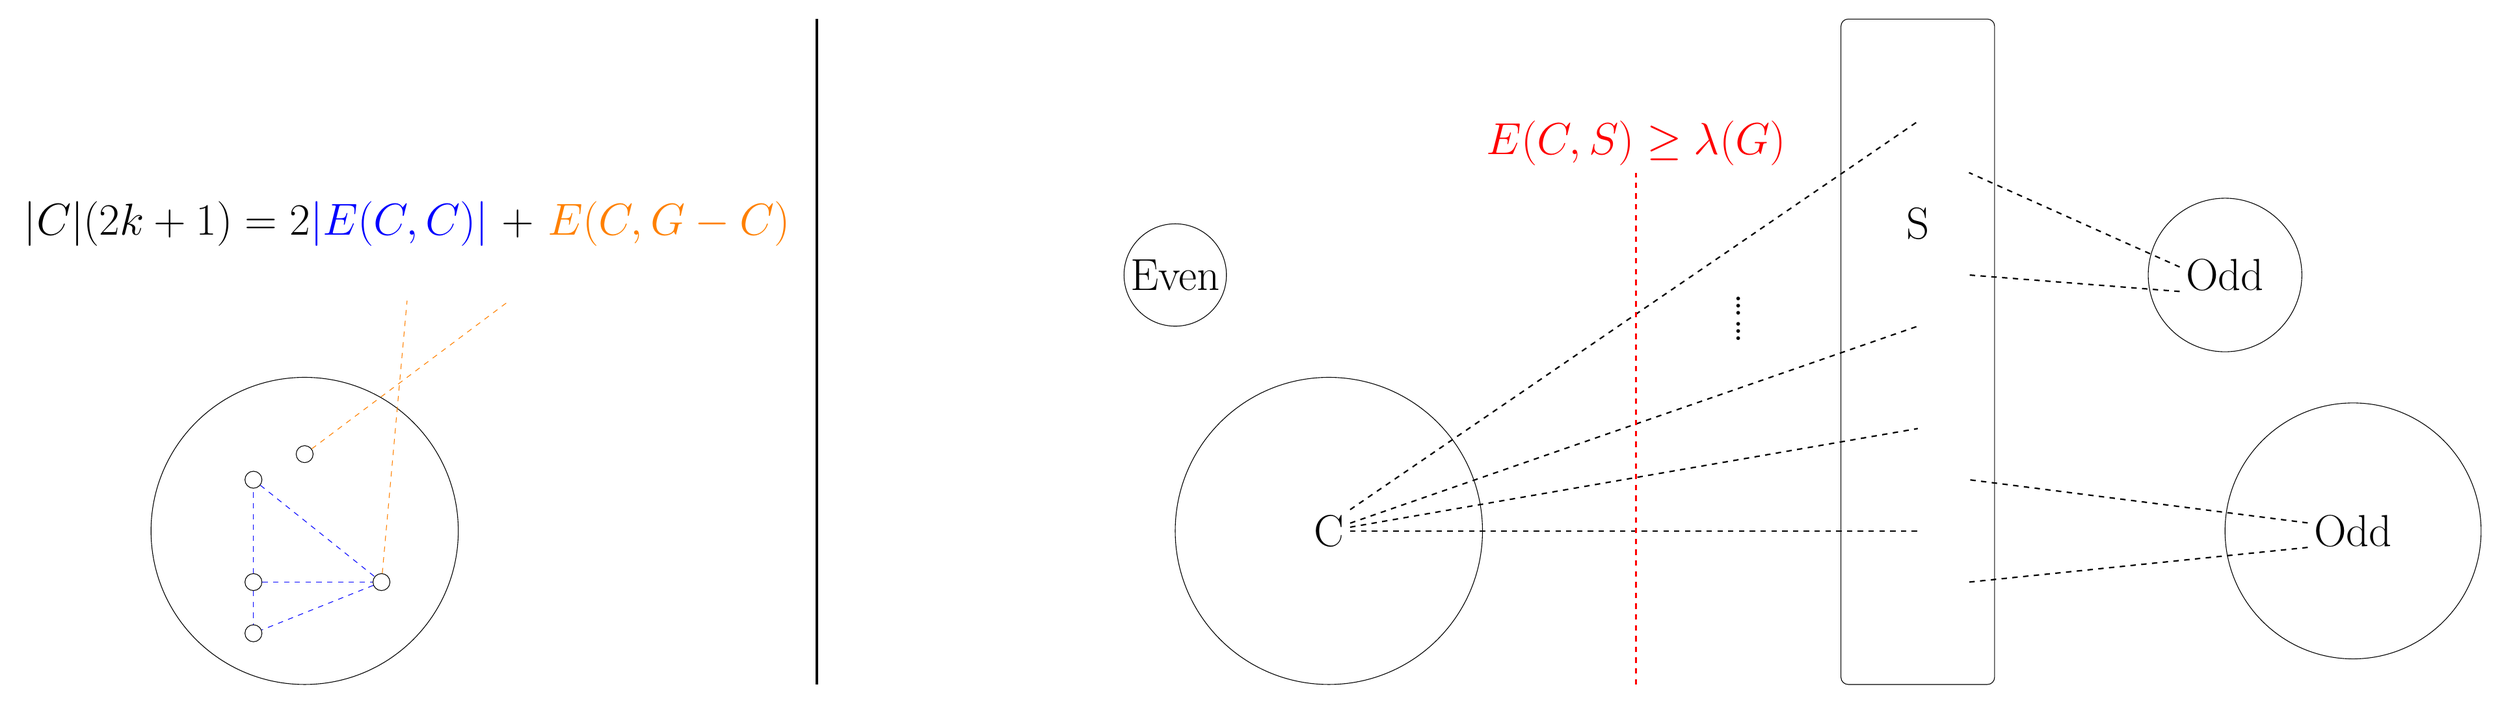
\begin{tikzpicture}
            % LHS Drawing
            \draw (0,0) circle (3cm);
            \node[circle, draw = black] (node-1) at (-1,-1) {};
            \node[circle, draw = black] (node-2) at (-1,1) {};
            \node[circle, draw = black] (node-3) at (1.5,-1) {};
            \node[circle, draw = black] (node-4) at (-1,-2) {};
            \node[circle, draw = black] (node-5) at (0,1.5) {};
            \draw[dashed, blue] (node-1) -- (node-2);
            \draw[dashed, blue] (node-1) -- (node-3);
            \draw[dashed, blue] (node-1) -- (node-4);
            \draw[dashed, blue] (node-2) -- (node-3);
            \draw[dashed, blue] (node-3) -- (node-4);
            \draw[dashed, orange] (node-3) -- (2,4.5);
            \draw[dashed, orange] (node-5) -- (4,4.5);
            \node at (2, 6.0) {\Huge $|C|(2k + 1) = 2$\textcolor{blue}{$|E(C,C)|$} + \textcolor{orange}{$E(C, G-C)$}};

            % Separating Line
            \draw[very thick] (10, -3) -- (10, 10);

            % RHS Drawing
            \draw (20, 0) circle (3cm) node (C) {\Huge C};
            \draw (17, 5) circle (1cm) node {\Huge Even};
            \draw[rounded corners] (30, -3) rectangle (33, 10);
            \node at (31.5, 6) {\Huge S};
            \draw(40, 0) circle (2.5cm) node (N1) {\Huge Odd};
            \draw(37.5, 5) circle (1.5cm) node (N2) {\Huge Odd};
            \draw[dashed, thick] (C.0) -- (31.5, 0);
            \draw[dashed, thick] (C.10) -- (31.5, 2);
            \draw[dashed, thick] (C.20) -- (31.5, 4);
            \draw[dashed, thick] (C.45) -- (31.5, 8);
            \draw[dashed, thick] (N2.200) -- (32.5, 5);
            \draw[dashed, thick] (N2.170) -- (32.5, 7);
            \draw[dashed, thick] (N1.200) -- (32.5, -1);
            \draw[dashed, thick] (N1.170) -- (32.5, 1);
            \node at (28, 4.5) {\Huge $\vdots$};
            \node at (28, 4) {\Huge $\vdots$};
            \draw[very thick, red, dashed] (26, -3) -- (26, 7) node[text=red,anchor=south] {\Huge $E(C, S) \geq \lambda(G)$};
        \end{tikzpicture}
    }
\end{figure}

\end{document}
